\documentclass[11pt,a4paper]{article}
\usepackage[utf8]{inputenc}
\usepackage[margin=1in]{geometry}
\usepackage{amsmath,amsfonts,amssymb}
\usepackage{graphicx}
\usepackage{tikz}
\usepackage{pgfgantt}
\usepackage{booktabs}
\usepackage{array}
\usepackage{enumitem}
\usepackage{xcolor}
\usepackage{hyperref}
\usepackage{fancyhdr}
\usepackage{titlesec}

% Colors
\definecolor{bankBlue}{RGB}{0,123,255}
\definecolor{bankLightBlue}{RGB}{52,152,219}
\definecolor{bankGreen}{RGB}{40,167,69}
\definecolor{bankOrange}{RGB}{255,193,7}

% Header and footer
\pagestyle{fancy}
\fancyhf{}
\fancyhead[L]{Bank of React - Project Document}
\fancyhead[R]{Version 1.0}
\fancyfoot[C]{\thepage}

% Title formatting
\titleformat{\section}{\Large\bfseries\color{bankBlue}}{\thesection}{1em}{}
\titleformat{\subsection}{\large\bfseries\color{bankLightBlue}}{\thesubsection}{1em}{}
\titleformat{\subsubsection}{\normalsize\bfseries\color{bankBlue}}{\thesubsubsection}{1em}{}

% Hyperlink setup
\hypersetup{
    colorlinks=true,
    linkcolor=bankBlue,
    urlcolor=bankOrange,
    citecolor=bankLightBlue
}

\begin{document}

% Title page
\begin{titlepage}
\centering
\vspace*{2cm}

{\Huge\bfseries\color{bankBlue} Bank of React}\\[0.5cm]
{\Large Project Document}\\[2cm]

\begin{tabular}{ll}
\textbf{Assignment:} & Assignment 3 - Bank of React \\
\textbf{Start Date:} & October 15, 2025 \\
\textbf{Due Date:} & November 3, 2025, 11:59 PM \\
\textbf{Project Duration:} & 3 weeks (19 days) \\
\textbf{Team Size:} & 2 developers (David \& Kevin) \\
\textbf{Document Version:} & 1.0 \\
\textbf{Last Updated:} & November 2, 2025 \\
\end{tabular}

\vfill

{\large A React-based banking application with dual bank support, client-side routing, and authentication.}

\end{titlepage}

% Table of Contents
\tableofcontents
\newpage

\section{Feature Requirements}

\subsection{Core Features}

\subsubsection{Landing Page}
\begin{itemize}[leftmargin=*]
    \item \textbf{Multi-Bank Access}: Landing page allowing users to choose between David's Bank and Kevin's Bank
    \item \textbf{Navigation}: Clean interface with links to both banking portals
    \item \textbf{User-Friendly Design}: Simple, intuitive card-based layout
\end{itemize}

\subsubsection{Bank Portal Features (Per Bank)}
\begin{itemize}[leftmargin=*]
    \item \textbf{Home Page}: Display account balance and navigation menu
    \item \textbf{User Profile}: Display user information (username, email, member since date)
    \item \textbf{Login System}: Form-based authentication with validation
    \item \textbf{Credits Management}: View credit history, add new credits
    \item \textbf{Debits Management}: View debit history, add new debits
    \item \textbf{Account Balance}: Dynamic calculation based on credits and debits
\end{itemize}

\subsubsection{Authentication System}
\begin{itemize}[leftmargin=*]
    \item \textbf{Login Required}: Users must authenticate before accessing bank features
    \item \textbf{Form Validation}: Username and password validation
    \item \textbf{Email Support}: Optional email field in login form
    \item \textbf{Separate Auth States}: Independent authentication for each bank
    \item \textbf{Automatic Redirect}: Unauthenticated users redirected to login
\end{itemize}

\subsubsection{State Management}
\begin{itemize}[leftmargin=*]
    \item \textbf{Separate Bank States}: Independent credits, debits, and balances for each bank
    \item \textbf{User Data Isolation}: Separate user profiles per bank
    \item \textbf{Independent Calculations}: Balance calculations separate for each bank
    \item \textbf{Transaction History}: Separate transaction histories maintained per bank
\end{itemize}

\subsection{Technical Requirements}

\subsubsection{React Router Implementation}
\begin{itemize}[leftmargin=*]
    \item Use of \texttt{BrowserRouter} for client-side routing
    \item Use of \texttt{Route} component for defining routes
    \item Use of \texttt{Link} component for navigation
    \item Use of \texttt{Redirect} component for programmatic navigation
    \item Route protection based on authentication state
\end{itemize}

\subsubsection{React Components}
\begin{itemize}[leftmargin=*]
    \item Component-based architecture
    \item Props passing for data flow
    \item State management in App component
    \item Lifecycle methods (\texttt{componentDidMount})
    \item Event handlers for user interactions
    \item Controlled components for form inputs
\end{itemize}

\subsubsection{Data Fetching}
\begin{itemize}[leftmargin=*]
    \item API integration using \texttt{fetch}
    \item Async/await for asynchronous operations
    \item Error handling for API requests
    \item Data initialization on component mount
\end{itemize}

\subsubsection{Component Organization}
\begin{itemize}[leftmargin=*]
    \item Prefixed components (\texttt{kevin\_} and \texttt{david\_})
    \item Shared core logic with different styling
    \item Modular component structure
    \item Reusable component patterns
\end{itemize}

\subsection{Version Control Requirements}

\subsubsection{Git Workflow}
\begin{itemize}[leftmargin=*]
    \item \textbf{Feature Branches}: Separate branch for each major feature
    \item \textbf{Pull Requests}: Merge feature branches via pull requests
    \item \textbf{Commit Practices}: Small, frequent commits with descriptive messages
    \item \textbf{Branch Naming}: Clear, descriptive branch names (e.g., feat/my-home-page, feat/user-auth-enhancements)
\end{itemize}

\subsection{Deployment Requirements}

\begin{itemize}[leftmargin=*]
    \item Website deployed to GitHub Pages
    \item Live URL accessible and functional
    \item README includes link to deployed site
    \item All features working in production environment
    \item Proper basename configuration for GitHub Pages
\end{itemize}

\section{Application Architecture Description and Diagram}

\subsection{Architecture Overview}

The Bank of React application follows a \textbf{React-based Single-Page Application (SPA) architecture} using React Router for client-side routing. The architecture emphasizes \textbf{component-based development}, \textbf{state management}, and \textbf{authentication-based route protection}.

\subsection{System Components}

\subsubsection{Presentation Layer (React Components)}
\begin{itemize}[leftmargin=*]
    \item \textbf{Landing Page}: Entry point with bank selection
    \item \textbf{Home Components}: Display account balance and navigation (separate for each bank)
    \item \textbf{User Profile Components}: Display user information (separate for each bank)
    \item \textbf{Login Components}: Authentication forms with validation (separate for each bank)
    \item \textbf{Credits Components}: Credit management interface (separate for each bank)
    \item \textbf{Debits Components}: Debit management interface (separate for each bank)
    \item \textbf{Account Balance Components}: Balance display (separate for each bank)
\end{itemize}

\subsubsection{Routing Layer (React Router)}
\begin{itemize}[leftmargin=*]
    \item \textbf{Router}: BrowserRouter wrapper for entire application
    \item \textbf{Routes}: Defined routes for all page views
    \item \textbf{Protected Routes}: Authentication-based access control
    \item \textbf{Navigation}: Link components for user navigation
    \item \textbf{Redirects}: Programmatic navigation after login
\end{itemize}

\subsubsection{State Management Layer (App Component)}
\begin{itemize}[leftmargin=*]
    \item \textbf{Kevin's Bank State}:
        \begin{itemize}
            \item \texttt{kevinCredits}: Array of credit transactions
            \item \texttt{kevinDebits}: Array of debit transactions
            \item \texttt{kevinBalance}: Calculated account balance
            \item \texttt{kevinAuthenticated}: Authentication status
            \item \texttt{kevinUser}: User profile data
        \end{itemize}
    \item \textbf{David's Bank State}:
        \begin{itemize}
            \item \texttt{davidCredits}: Array of credit transactions
            \item \texttt{davidDebits}: Array of debit transactions
            \item \texttt{davidBalance}: Calculated account balance
            \item \texttt{davidAuthenticated}: Authentication status
            \item \texttt{davidUser}: User profile data
        \end{itemize}
\end{itemize}

\subsubsection{Business Logic Layer}
\begin{itemize}[leftmargin=*]
    \item \textbf{Balance Calculation}: Separate functions for each bank
    \item \textbf{Transaction Management}: Add credit/debit functions per bank
    \item \textbf{Authentication Handlers}: Login functions per bank
    \item \textbf{API Integration}: Data fetching on component mount
\end{itemize}

\subsection{Architecture Diagram}

\begin{figure}[h]
\centering
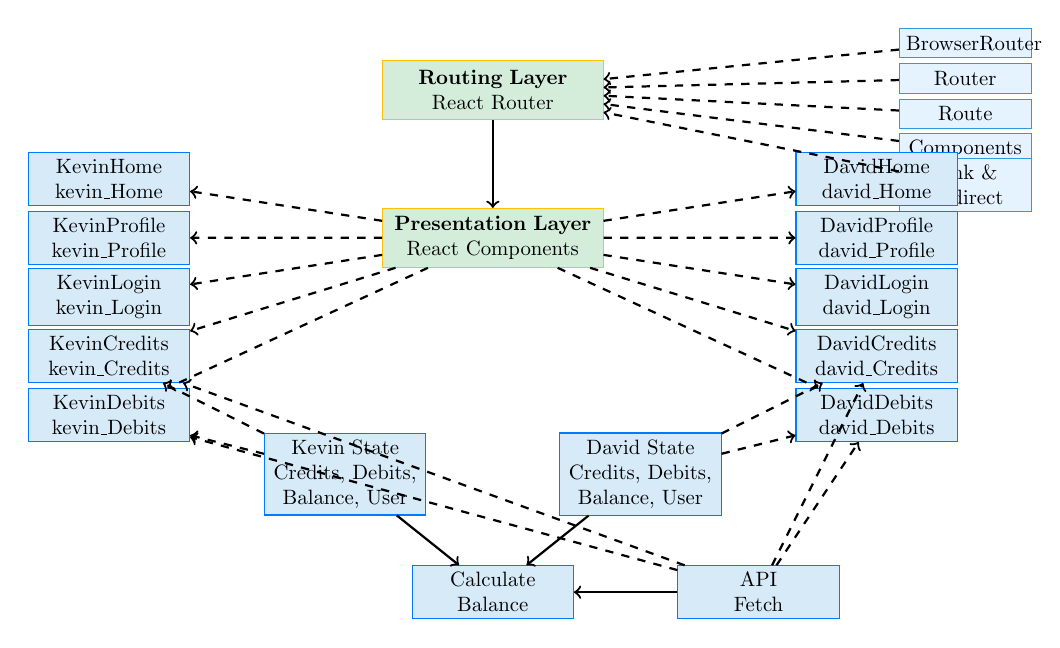
\begin{tikzpicture}[
    box/.style={rectangle, draw=bankBlue, fill=bankLightBlue!20, text width=2.5cm, text centered, minimum height=0.8cm},
    layer/.style={rectangle, draw=bankOrange, fill=bankGreen!20, text width=3.5cm, text centered, minimum height=1cm},
    small/.style={rectangle, draw=bankLightBlue, fill=bankBlue!10, text width=2cm, text centered, minimum height=0.5cm},
    scale=0.75,
    transform shape
]

% Main Layers (top)
\node[layer] (routing) at (0,8) {\textbf{Routing Layer}\\React Router};
\node[layer] (presentation) at (0,5.5) {\textbf{Presentation Layer}\\React Components};

% Routing Components (stacked on far right, well spaced)
\node[small] (router) at (8,8.8) {BrowserRouter};
\node[small] (route_comp) at (8,8.2) {Router};
\node[small] (routes) at (8,7.6) {Route};
\node[small] (comp) at (8,7.0) {Components};
\node[small] (links) at (8,6.4) {Link \&\\Redirect};

% Presentation Components - Kevin (left column, well spaced)
\node[box] (khome) at (-6.5,6.5) {KevinHome\\kevin\_Home};
\node[box] (kprofile) at (-6.5,5.5) {KevinProfile\\kevin\_Profile};
\node[box] (klogin) at (-6.5,4.5) {KevinLogin\\kevin\_Login};
\node[box] (kcredits) at (-6.5,3.5) {KevinCredits\\kevin\_Credits};
\node[box] (kdebits) at (-6.5,2.5) {KevinDebits\\kevin\_Debits};

% Presentation Components - David (right column, well spaced)
\node[box] (dhome) at (6.5,6.5) {DavidHome\\david\_Home};
\node[box] (dprofile) at (6.5,5.5) {DavidProfile\\david\_Profile};
\node[box] (dlogin) at (6.5,4.5) {DavidLogin\\david\_Login};
\node[box] (dcredits) at (6.5,3.5) {DavidCredits\\david\_Credits};
\node[box] (ddebits) at (6.5,2.5) {DavidDebits\\david\_Debits};

% State Management (middle, between presentation and business logic)
\node[box] (kstate) at (-2.5,1.5) {Kevin State\\Credits, Debits,\\Balance, User};
\node[box] (dstate) at (2.5,1.5) {David State\\Credits, Debits,\\Balance, User};

% Business Logic (bottom)
\node[box] (calc) at (0,-0.5) {Calculate\\Balance};
\node[box] (api) at (4.5,-0.5) {API\\Fetch};

% Main flow connections (solid arrows)
\draw[->, thick] (routing) -- (presentation);
\draw[->, thick] (kstate) -- (calc);
\draw[->, thick] (dstate) -- (calc);
\draw[->, thick] (api) -- (calc);

% Routing connections (dashed arrows)
\draw[->, thick, dashed] (router) -- (routing);
\draw[->, thick, dashed] (route_comp) -- (routing);
\draw[->, thick, dashed] (routes) -- (routing);
\draw[->, thick, dashed] (comp) -- (routing);
\draw[->, thick, dashed] (links) -- (routing);

% Presentation to components (dashed arrows)
\draw[->, thick, dashed] (presentation) -- (khome);
\draw[->, thick, dashed] (presentation) -- (kprofile);
\draw[->, thick, dashed] (presentation) -- (klogin);
\draw[->, thick, dashed] (presentation) -- (kcredits);
\draw[->, thick, dashed] (presentation) -- (kdebits);
\draw[->, thick, dashed] (presentation) -- (dhome);
\draw[->, thick, dashed] (presentation) -- (dprofile);
\draw[->, thick, dashed] (presentation) -- (dlogin);
\draw[->, thick, dashed] (presentation) -- (dcredits);
\draw[->, thick, dashed] (presentation) -- (ddebits);

% State to components (dashed arrows)
\draw[->, thick, dashed] (kstate) -- (kcredits);
\draw[->, thick, dashed] (kstate) -- (kdebits);
\draw[->, thick, dashed] (dstate) -- (dcredits);
\draw[->, thick, dashed] (dstate) -- (ddebits);

% API to components (dashed arrows)
\draw[->, thick, dashed] (api) -- (kcredits);
\draw[->, thick, dashed] (api) -- (kdebits);
\draw[->, thick, dashed] (api) -- (dcredits);
\draw[->, thick, dashed] (api) -- (ddebits);

\end{tikzpicture}
\caption{Bank of React Application Architecture}
\end{figure}

\subsection{Data Flow}

\begin{enumerate}[leftmargin=*]
    \item \textbf{User Navigation}: User selects bank from landing page
    \item \textbf{Route Matching}: React Router matches URL to route definition
    \item \textbf{Authentication Check}: System checks authentication state
    \item \textbf{Component Rendering}: Appropriate component rendered (bank portal or login)
    \item \textbf{State Access}: Component accesses relevant bank state from App
    \item \textbf{User Interaction}: User performs actions (add transaction, login, etc.)
    \item \textbf{State Update}: App component state updated via handler functions
    \item \textbf{UI Update}: Component re-renders with new data
\end{enumerate}

\subsection{Technology Stack}

\begin{itemize}[leftmargin=*]
    \item \textbf{React 17.0.2}: Component-based UI library
    \item \textbf{React Router 5.3.0}: Client-side routing
    \item \textbf{JavaScript (ES6+)}: Application logic
    \item \textbf{Fetch API}: HTTP requests for data
    \item \textbf{Git}: Version control
    \item \textbf{GitHub}: Repository hosting
    \item \textbf{GitHub Pages}: Static website hosting
\end{itemize}

\subsection{Key Design Patterns}

\begin{itemize}[leftmargin=*]
    \item \textbf{Component Composition}: Breaking UI into reusable components
    \item \textbf{State Lifting}: Centralized state management in App component
    \item \textbf{Unidirectional Data Flow}: Props down, events up
    \item \textbf{Route Protection}: Conditional rendering based on authentication
    \item \textbf{Separation of Concerns}: Logic separated from presentation
    \item \textbf{DRY Principle}: Shared logic with different styling per bank
\end{itemize}

\section{Epics, User Stories, and Acceptance Criteria}

\subsection{Epic 1: Landing Page and Multi-Bank Access}

\subsubsection{User Story 1.1: Landing Page with Bank Selection}
\textbf{As a} user\\
\textbf{I want to} see a landing page with options to access different banks\\
\textbf{So that} I can choose which banking portal to use

\textbf{Acceptance Criteria:}
\begin{itemize}[leftmargin=*]
    \item Landing page displays at root route (\texttt{/})
    \item Page shows options for David's Bank and Kevin's Bank
    \item Each bank option has a clear call-to-action button
    \item Navigation links correctly route to respective bank portals
    \item Design is clean and user-friendly
\end{itemize}

\subsection{Epic 2: Authentication System}

\subsubsection{User Story 2.1: Login Form with Validation}
\textbf{As a} user\\
\textbf{I want to} log in with username and password\\
\textbf{So that} I can access my bank account

\textbf{Acceptance Criteria:}
\begin{itemize}[leftmargin=*]
    \item Login form includes username and password fields
    \item Form includes optional email field
    \item Username and password are required fields
    \item Validation errors display when fields are empty
    \item Error messages clear when user starts typing
    \item Form submission triggers authentication
\end{itemize}

\subsubsection{User Story 2.2: Authentication Protection}
\textbf{As a} user\\
\textbf{I want to} be required to log in before accessing bank features\\
\textbf{So that} my account is secure

\textbf{Acceptance Criteria:}
\begin{itemize}[leftmargin=*]
    \item Unauthenticated users accessing bank routes see login form
    \item Login sets authentication state for respective bank
    \item Authentication state is separate for each bank
    \item After login, users can access bank features
    \item Login redirects to appropriate bank home page
\end{itemize}

\subsection{Epic 3: Home Page and Navigation}

\subsubsection{User Story 3.1: Home Page Display}
\textbf{As a} user\\
\textbf{I want to} see my account balance on the home page\\
\textbf{So that} I can quickly view my financial status

\textbf{Acceptance Criteria:}
\begin{itemize}[leftmargin=*]
    \item Home page displays after successful authentication
    \item Account balance is prominently displayed
    \item Balance is calculated correctly (Credits - Debits)
    \item Balance shows 2 decimal places
    \item Navigation links to other pages are available
\end{itemize}

\subsubsection{User Story 3.2: Navigation Menu}
\textbf{As a} user\\
\textbf{I want to} navigate between different bank pages\\
\textbf{So that} I can access all bank features easily

\textbf{Acceptance Criteria:}
\begin{itemize}[leftmargin=*]
    \item Navigation links present on home page
    \item Links to User Profile, Login, Credits, and Debits
    \item Links use React Router's Link component
    \item Navigation works correctly and updates URL
    \item Users can return to home from other pages
\end{itemize}

\subsection{Epic 4: User Profile}

\subsubsection{User Story 4.1: View User Profile}
\textbf{As a} user\\
\textbf{I want to} view my profile information\\
\textbf{So that} I can see my account details

\textbf{Acceptance Criteria:}
\begin{itemize}[leftmargin=*]
    \item Profile page displays username
    \item Profile page displays email (if provided)
    \item Profile page displays member since date
    \item Information is styled and easy to read
    \item Link to return to home is available
\end{itemize}

\subsection{Epic 5: Credits Management}

\subsubsection{User Story 5.1: View Credits History}
\textbf{As a} user\\
\textbf{I want to} view all my credit transactions\\
\textbf{So that} I can see my income history

\textbf{Acceptance Criteria:}
\begin{itemize}[leftmargin=*]
    \item Credits page displays list of all credits
    \item Each credit shows description, amount, and date
    \item Credits from API are loaded on page load
    \item Amounts display with 2 decimal places
    \item Dates display in yyyy-mm-dd format
\end{itemize}

\subsubsection{User Story 5.2: Add New Credit}
\textbf{As a} user\\
\textbf{I want to} add new credit transactions\\
\textbf{So that} I can record income

\textbf{Acceptance Criteria:}
\begin{itemize}[leftmargin=*]
    \item Form to add new credit with description and amount fields
    \item Form validation ensures required fields are filled
    \item New credit added to credit list immediately
    \item New credit includes current date (yyyy-mm-dd)
    \item Account balance updates automatically after adding credit
    \item Form clears after successful submission
\end{itemize}

\subsection{Epic 6: Debits Management}

\subsubsection{User Story 6.1: View Debits History}
\textbf{As a} user\\
\textbf{I want to} view all my debit transactions\\
\textbf{So that} I can see my spending history

\textbf{Acceptance Criteria:}
\begin{itemize}[leftmargin=*]
    \item Debits page displays list of all debits
    \item Each debit shows description, amount, and date
    \item Debits from API are loaded on page load
    \item Amounts display with 2 decimal places
    \item Dates display in yyyy-mm-dd format
\end{itemize}

\subsubsection{User Story 6.2: Add New Debit}
\textbf{As a} user\\
\textbf{I want to} add new debit transactions\\
\textbf{So that} I can record expenses

\textbf{Acceptance Criteria:}
\begin{itemize}[leftmargin=*]
    \item Form to add new debit with description and amount fields
    \item Form validation ensures required fields are filled
    \item New debit added to debit list immediately
    \item New debit includes current date (yyyy-mm-dd)
    \item Account balance updates automatically after adding debit
    \item Form clears after successful submission
\end{itemize}

\subsection{Epic 7: Account Balance Calculation}

\subsubsection{User Story 7.1: Dynamic Balance Calculation}
\textbf{As a} user\\
\textbf{I want to} see my account balance calculated from credits and debits\\
\textbf{So that} I know my current financial status

\textbf{Acceptance Criteria:}
\begin{itemize}[leftmargin=*]
    \item Balance = Total Credits - Total Debits
    \item Balance updates automatically when transactions added
    \item Balance can be negative if debits exceed credits
    \item Balance displays with 2 decimal places
    \item Balance displayed on Home, Credits, and Debits pages
\end{itemize}

\subsection{Epic 8: Dual Bank System}

\subsubsection{User Story 8.1: Separate Bank States}
\textbf{As a} developer\\
\textbf{I want to} maintain separate state for each bank\\
\textbf{So that} banks operate independently

\textbf{Acceptance Criteria:}
\begin{itemize}[leftmargin=*]
    \item Kevin's and David's banks have separate credit arrays
    \item Kevin's and David's banks have separate debit arrays
    \item Kevin's and David's banks have separate balance calculations
    \item Transactions in one bank don't affect the other
    \item Each bank maintains independent authentication state
\end{itemize}

\subsection{Epic 9: Code Quality and Version Control}

\subsubsection{User Story 9.1: Feature Branch Workflow}
\textbf{As a} developer\\
\textbf{I want to} create feature branches for each feature\\
\textbf{So that} I can develop features in isolation

\textbf{Acceptance Criteria:}
\begin{itemize}[leftmargin=*]
    \item Each major feature has its own branch
    \item Branch names follow convention (feat/feature-name)
    \item Feature branches merged via pull requests
    \item Commit messages are descriptive and clear
    \item Code is well-organized and commented
\end{itemize}

\section{Project Schedule Chart (Gantt Chart)}

\subsection{Project Timeline Overview}

\textbf{Project Duration}: 3 weeks (19 days)\\
\textbf{Start Date}: October 15, 2025\\
\textbf{Due Date}: November 3, 2025, 11:59 PM\\
\textbf{Team Size}: 2 developers (David \& Kevin)

\subsection{Detailed Gantt Chart}

\begin{figure}[h]
\centering
\begin{ganttchart}[
    x unit=0.5cm,
    y unit title=0.6cm,
    y unit chart=0.5cm,
    vgrid,
    hgrid,
    title label font=\bfseries\footnotesize,
    bar label font=\footnotesize,
    group label font=\small,
    milestone label font=\footnotesize,
    bar/.append style={fill=bankLightBlue!80},
    milestone/.append style={fill=bankOrange,rounded corners=2pt},
    group/.append style={fill=bankBlue!60}
]{1}{19}

\gantttitle{Bank of React Project Timeline}{19} \\
\gantttitle{October}{16}
\gantttitle{November}{3} \\
\gantttitlelist{15,16,17,18,19,20,21,22,23,24,25,26,27,28,29,30,31,1,2}{1} \\

\ganttgroup{Planning \& Setup}{1}{3} \\
\ganttbar{Project Planning}{1}{2} \\
\ganttbar{Repository Setup}{1}{2} \\
\ganttbar{Starter Code Review}{2}{3} \\
\ganttbar{Project Document Draft}{2}{3} \\

\ganttgroup{Landing Page \& Routing}{3}{6} \\
\ganttbar{Landing Page Component}{3}{4} \\
\ganttbar{Router Setup}{4}{5} \\
\ganttbar{Multi-Bank Routing}{5}{6} \\

\ganttgroup{Authentication System}{6}{9} \\
\ganttbar{Login Components}{6}{7} \\
\ganttbar{Form Validation}{7}{8} \\
\ganttbar{Route Protection}{8}{9} \\

\ganttgroup{Credits \& Debits}{9}{14} \\
\ganttbar{Credits Component}{9}{11} \\
\ganttbar{Debits Component}{11}{13} \\
\ganttbar{API Integration}{10}{12} \\
\ganttbar{Transaction Forms}{12}{14} \\

\ganttgroup{Dual Bank System}{14}{16} \\
\ganttbar{State Separation}{14}{15} \\
\ganttbar{Component Prefixing}{15}{16} \\
\ganttbar{Independent Calculations}{15}{16} \\

\ganttgroup{Testing \& Deployment}{16}{19} \\
\ganttbar{Testing \& Bug Fixes}{16}{17} \\
\ganttbar{Code Review \& Cleanup}{17}{18} \\
\ganttbar{Final Documentation}{18}{19} \\
\ganttbar{GitHub Pages Deploy}{18}{19} \\
\ganttbar{PDF \& Submission Prep}{19}{19} \\

\ganttmilestone{Setup Complete}{3} \\
\ganttmilestone{Routing Complete}{6} \\
\ganttmilestone{Auth Complete}{9} \\
\ganttmilestone{Features Complete}{14} \\
\ganttmilestone{Dual Bank Complete}{16} \\
\ganttmilestone{Project Due}{19}

\end{ganttchart}
\caption{Project Timeline - Gantt Chart (Oct 15 - Nov 3, 2025)}
\end{figure}

\subsection{Phase Breakdown}

\subsubsection{Phase 1: Planning \& Setup (Days 1-3, Oct 15-17)}
\textbf{Tasks:}
\begin{itemize}[leftmargin=*]
    \item Review assignment requirements
    \item Analyze starter code structure
    \item Set up GitHub repository
    \item Review React Router documentation
    \item Draft project document structure
\end{itemize}

\textbf{Deliverables:}
\begin{itemize}[leftmargin=*]
    \item Project document outline
    \item GitHub repository configured
    \item Starter code imported and reviewed
\end{itemize}

\subsubsection{Phase 2: Landing Page \& Routing (Days 3-6, Oct 17-20)}
\textbf{Tasks:}
\begin{itemize}[leftmargin=*]
    \item Create LandingPage component
    \item Set up React Router
    \item Configure routes for both banks
    \item Test navigation between pages
\end{itemize}

\textbf{Deliverables:}
\begin{itemize}[leftmargin=*]
    \item Working landing page
    \item Router configuration
    \item Basic routing between banks
\end{itemize}

\textbf{Branches:}
\begin{itemize}[leftmargin=*]
    \item \texttt{feat/my-home-page}
\end{itemize}

\subsubsection{Phase 3: Authentication System (Days 6-9, Oct 20-23)}
\textbf{Tasks:}
\begin{itemize}[leftmargin=*]
    \item Create Login components (Kevin and David versions)
    \item Implement form validation
    \item Add authentication state management
    \item Implement route protection
    \item Test authentication flow
\end{itemize}

\textbf{Deliverables:}
\begin{itemize}[leftmargin=*]
    \item Working login forms
    \item Form validation
    \item Protected routes
    \item Authentication state management
\end{itemize}

\textbf{Branches:}
\begin{itemize}[leftmargin=*]
    \item \texttt{feat/user-auth-enhancements}
\end{itemize}

\subsubsection{Phase 4: Credits \& Debits (Days 9-14, Oct 23-28)}
\textbf{Tasks:}
\begin{itemize}[leftmargin=*]
    \item Create Credits components (Kevin and David versions)
    \item Create Debits components (Kevin and David versions)
    \item Integrate API endpoints
    \item Implement add transaction functionality
    \item Implement balance calculation
    \item Test transaction flows
\end{itemize}

\textbf{Deliverables:}
\begin{itemize}[leftmargin=*]
    \item Working Credits pages
    \item Working Debits pages
    \item API integration complete
    \item Transaction addition working
    \item Balance calculation working
\end{itemize}

\textbf{Branches:}
\begin{itemize}[leftmargin=*]
    \item Feature branches for Credits and Debits
\end{itemize}

\subsubsection{Phase 5: Dual Bank System (Days 14-16, Oct 28-30)}
\textbf{Tasks:}
\begin{itemize}[leftmargin=*]
    \item Separate state management per bank
    \item Split components with prefixes
    \item Independent balance calculations
    \item Separate authentication states
    \item Test bank independence
\end{itemize}

\textbf{Deliverables:}
\begin{itemize}[leftmargin=*]
    \item Completely separate bank states
    \item Independent transaction histories
    \item Separate user profiles
    \item Verified bank isolation
\end{itemize}

\textbf{Branches:}
\begin{itemize}[leftmargin=*]
    \item \texttt{feat/user-auth-enhancements}
\end{itemize}

\subsubsection{Phase 6: Testing, Documentation \& Deployment (Days 16-19, Oct 30-Nov 3)}
\textbf{Tasks:}
\begin{itemize}[leftmargin=*]
    \item Comprehensive testing of all features
    \item Cross-browser testing
    \item Code cleanup and refactoring
    \item Add code comments
    \item Complete project document
    \item Update README with team info and deployment link
    \item Deploy to GitHub Pages
    \item Final testing of deployed site
    \item Prepare submission materials (PDF conversion)
\end{itemize}

\textbf{Deliverables:}
\begin{itemize}[leftmargin=*]
    \item Fully tested application
    \item Clean, commented code
    \item Complete project document (PDF)
    \item Updated README
    \item Live website on GitHub Pages
    \item Submission ready for Brightspace
\end{itemize}

\subsection{Milestones}

\begin{itemize}[leftmargin=*]
    \item \textbf{October 17}: Project setup and planning complete
    \item \textbf{October 20}: Landing page and routing complete
    \item \textbf{October 23}: Authentication system complete
    \item \textbf{October 28}: Credits and Debits features complete
    \item \textbf{October 30}: Dual bank system complete
    \item \textbf{November 3}: Project deployed, tested, and submitted
\end{itemize}

\subsection{Risk Management}

\subsubsection{Identified Risks}
\begin{itemize}[leftmargin=*]
    \item \textbf{State Management Complexity}: Managing separate states for two banks
    \item \textbf{Route Protection Logic}: Ensuring proper authentication checks
    \item \textbf{API Integration Issues}: Handling API errors and loading states
    \item \textbf{Balance Calculation Errors}: Ensuring accurate financial calculations
    \item \textbf{Merge Conflicts}: Multiple feature branches may conflict
    \item \textbf{Time Constraints}: 3 weeks is a tight timeline
\end{itemize}

\subsubsection{Mitigation Strategies}
\begin{itemize}[leftmargin=*]
    \item \textbf{Incremental Development}: Build and test one feature at a time
    \item \textbf{State Isolation}: Clear separation of bank states
    \item \textbf{Error Handling}: Comprehensive error handling for API calls
    \item \textbf{Testing}: Test balance calculations with various scenarios
    \item \textbf{Small Commits}: Make frequent, small commits to minimize conflicts
    \item \textbf{Early Start}: Begin project as soon as assigned
    \item \textbf{Code Reviews}: Review pull requests carefully before merging
\end{itemize}

\subsection{Resource Allocation}

\subsubsection{Team Structure (2-person team)}
\begin{itemize}[leftmargin=*]
    \item \textbf{David}: Landing page, David's bank components, styling
    \item \textbf{Kevin}: Kevin's bank components, authentication, routing
    \item \textbf{Shared}: State management, API integration, testing, documentation
\end{itemize}

\subsubsection{Recommended Task Division}
\begin{itemize}[leftmargin=*]
    \item \textbf{Developer 1}: Landing page, routing setup, Credits/Debits components
    \item \textbf{Developer 2}: Authentication, state management, User Profile, balance calculations
    \item \textbf{Both}: Testing, code review, documentation, deployment
\end{itemize}

\subsubsection{Required Tools}
\begin{itemize}[leftmargin=*]
    \item \textbf{Text Editor/IDE}: VS Code or similar
    \item \textbf{Web Browser}: Chrome, Firefox, or Edge with DevTools
    \item \textbf{Node.js \& npm}: For React development
    \item \textbf{Git}: For version control
    \item \textbf{GitHub Account}: For repository hosting and Pages
    \item \textbf{LaTeX Editor}: For project document (Overleaf, TeXShop, etc.)
\end{itemize}

\section{Implementation Notes}

\subsection{React Router Implementation}

\subsubsection{Setting Up Router}
\begin{itemize}[leftmargin=*]
    \item Import \texttt{BrowserRouter as Router} from \texttt{react-router-dom}
    \item Wrap application in \texttt{<Router>} component
    \item Use \texttt{basename="/Bank-of-React"} for GitHub Pages
    \item Define routes using \texttt{<Route>} components
    \item Use \texttt{exact} prop for precise path matching
\end{itemize}

\subsubsection{Navigation}
\begin{itemize}[leftmargin=*]
    \item Use \texttt{<Link to="/path">} for declarative navigation
    \item Use \texttt{<Redirect to="/path">} for programmatic navigation
    \item Pass props to routes using \texttt{render} prop
    \item Protect routes with conditional rendering based on auth state
\end{itemize}

\subsection{State Management}

\subsubsection{App Component State Structure}
\begin{verbatim}
state = {
  // Kevin's bank state
  kevinCredits: [],
  kevinDebits: [],
  kevinBalance: 0,
  kevinAuthenticated: false,
  kevinUser: {
    userName: 'Kevin User',
    email: 'kevin@example.com',
    memberSince: '11/22/99'
  },
  // David's bank state
  davidCredits: [],
  davidDebits: [],
  davidBalance: 0,
  davidAuthenticated: false,
  davidUser: {
    userName: 'David User',
    email: 'david@example.com',
    memberSince: '01/15/20'
  }
}
\end{verbatim}

\subsubsection{Balance Calculation}
\begin{itemize}[leftmargin=*]
    \item Formula: \texttt{Balance = Total Credits - Total Debits}
    \item Use \texttt{reduce()} to sum credits and debits
    \item Round to 2 decimal places using \texttt{toFixed(2)}
    \item Update balance after each transaction addition
    \item Separate calculation functions for each bank
\end{itemize}

\subsection{API Integration}

\subsubsection{Data Fetching}
\begin{itemize}[leftmargin=*]
    \item Use \texttt{async/await} in \texttt{componentDidMount()}
    \item Fetch from credits API: \texttt{https://johnnylaicode.github.io/api/credits.json}
    \item Fetch from debits API: \texttt{https://johnnylaicode.github.io/api/debits.json}
    \item Handle errors with try-catch blocks
    \item Initialize both banks with fetched data independently
\end{itemize}

\subsection{Component Organization}

\subsubsection{Component Naming Convention}
\begin{itemize}[leftmargin=*]
    \item Kevin's components: \texttt{kevin\_Home.js}, \texttt{kevin\_Credits.js}, etc.
    \item David's components: \texttt{david\_Home.js}, \texttt{david\_Credits.js}, etc.
    \item Shared logic with different styling
    \item Independent state management per bank
\end{itemize}

\subsection{Best Practices}

\begin{itemize}[leftmargin=*]
    \item \textbf{Component Structure}: Keep components focused and single-purpose
    \item \textbf{State Management}: Lift state up to App component when shared
    \item \textbf{Event Handling}: Use arrow functions for class methods
    \item \textbf{Form Handling}: Use controlled components with value and onChange
    \item \textbf{Validation}: Validate inputs before updating state
    \item \textbf{Error Handling}: Implement try-catch for async operations
    \item \textbf{Routing}: Use exact prop for precise route matching
    \item \textbf{Styling}: Inline styles for component-specific styling
    \item \textbf{Comments}: Add comments for complex logic
    \item \textbf{Git Workflow}: Create feature branches for each major feature
\end{itemize}

\section{API Endpoints}

\subsection{Credits API}
\begin{itemize}[leftmargin=*]
    \item \textbf{URL}: \texttt{https://johnnylaicode.github.io/api/credits.json}
    \item \textbf{Method}: GET
    \item \textbf{Response}: JSON array of credit objects
    \item \textbf{Credit Object Structure}:
        \begin{itemize}
            \item \texttt{id}: Unique identifier
            \item \texttt{description}: Credit description
            \item \texttt{amount}: Credit amount (number)
            \item \texttt{date}: Date in yyyy-mm-dd format
        \end{itemize}
\end{itemize}

\subsection{Debits API}
\begin{itemize}[leftmargin=*]
    \item \textbf{URL}: \texttt{https://johnnylaicode.github.io/api/debits.json}
    \item \textbf{Method}: GET
    \item \textbf{Response}: JSON array of debit objects
    \item \textbf{Debit Object Structure}:
        \begin{itemize}
            \item \texttt{id}: Unique identifier
            \item \texttt{description}: Debit description
            \item \texttt{amount}: Debit amount (number)
            \item \texttt{date}: Date in yyyy-mm-dd format
        \end{itemize}
\end{itemize}

\end{document}
